\documentclass{article}

\usepackage[T1]{fontenc}
\usepackage[utf8]{inputenc}
\usepackage[french]{babel}
\usepackage{array}
\usepackage{subcaption}
\usepackage[table]{xcolor}
\usepackage{graphicx}
\usepackage{listings}
\newcolumntype{M}[1]{>{\centering\arraybackslash}m{#1}}

\title{Rapport \LaTeX}
\author{Kyrian Balavoine}

\begin{document}

    \maketitle

    \begin{abstract}
        \textbf{Mosaic} est un jeu créé par \emph{Simon Tatham}. C'est un jeu type puzzle semblable à un démineur
    \end{abstract}
    \tableofcontents
    \section{Le jeu}

        \subsection{Règles}
        
            \begin{itemize}
                \item Chaque case du jeu peu être coloré en noir ou en blanc
                \item La contrainte d'une case est le chiffre indiqué dedans. Il concerne les case dans le carré 3x3 autoure de la contrainte.
                \item Une case est dite "satisfaite" si le nombre de case noir dans son entourage correspond à sa contrainte, et toute les autre case sont blanche
                \item Le jeu est gagné quand toute les cases sont satisfaites
            \end{itemize}

            \vspace{1cm}
            \clearpage
            Example :
            \begin{table}[ht]
                \subfloat[too much black]{
                \setlength\tabcolsep{0pt}
                \begin{tabular}{|@{\rule[-0.4cm]{0pt}{1cm}}*{3}{M{1cm} |}}
                    \hline
                    \cellcolor[HTML]{333333} & \cellcolor[HTML]{333333} &  \\
                    \hline
                        & \cellcolor[HTML]{333333}\textcolor{red}{3} & \cellcolor[HTML]{333333} \\
                    \hline
                        &  &  \\
                    \hline
                \end{tabular}}
                \quad
                \subfloat[too much white]{
                \setlength\tabcolsep{0pt}
                \begin{tabular}{|@{\rule[-0.4cm]{0pt}{1cm}}*{3}{M{1cm} |}}
                    \hline
                    \cellcolor[HTML]{333333} &  &  \\
                    \hline
                        & \textcolor{red}{3} & \cellcolor[HTML]{333333} \\
                    \hline
                        &  &  \\
                    \hline
                \end{tabular}}
                \quad
                \subfloat[perfect]{
                \setlength\tabcolsep{0pt}
                \begin{tabular}{|@{\rule[-0.4cm]{0pt}{1cm}}*{3}{M{1cm} |}}
                    \hline
                    \cellcolor[HTML]{333333} & \cellcolor[HTML]{333333} &  \\
                    \hline
                        & \textcolor{green!40!gray}{3} & \cellcolor[HTML]{333333} \\
                    \hline
                        &  &  \\
                    \hline
                \end{tabular}}
            \end{table}
        \subsection{La présentation}
            Par défaut, le jeu ressemble à ça quand on lance une partie :\\\\
            \label{game}
            \setlength\tabcolsep{0pt}
            \begin{tabular}{|@{\rule[-0.4cm]{0pt}{1cm}}*{5}{M{1cm} |}}
                \hline
                    0 &   &   & 3 &   \\
                \hline   
                      & 5 &   &   &   \\
                \hline   
                      &   & 4 &   & 1 \\
                \hline   
                    6 &   & 6 & 3 &   \\
                \hline   
                      &   &   &   &   \\
                \hline
            \end{tabular}
            \vspace{1cm}
            \\Cette même partie, une fois gagnée, ressemble à ça :\\
            \\\begin{tabular}{|@{\rule[-0.4cm]{0pt}{1cm}}*{5}{M{1cm} |}}
                \hline
                    \textcolor{green!40!gray}{0} &   & \cellcolor[HTML]{333333} & \textcolor{green!40!gray}{3} &   \\
                \hline   
                      & \textcolor{green!40!gray}{5} & \cellcolor[HTML]{333333} &   & \cellcolor[HTML]{333333} \\
                \hline   
                    \cellcolor[HTML]{333333} & \cellcolor[HTML]{333333} & \cellcolor[HTML]{333333}\textcolor{green!40!gray}4 &   & \textcolor{green!40!gray}{1} \\
                \hline   
                    \cellcolor[HTML]{333333}\textcolor{green!40!gray}{6} & \cellcolor[HTML]{333333} & \textcolor{green!40!gray}{6} & \textcolor{green!40!gray}{3} &   \\
                \hline   
                    \cellcolor[HTML]{333333} & \cellcolor[HTML]{333333} & \cellcolor[HTML]{333333} & \cellcolor[HTML]{333333} &   \\
                \hline
            \end{tabular}
        \subsection{notre jeu}
            avec mon binôme\cite{binome}, nous avons fait ce jeu :\\
            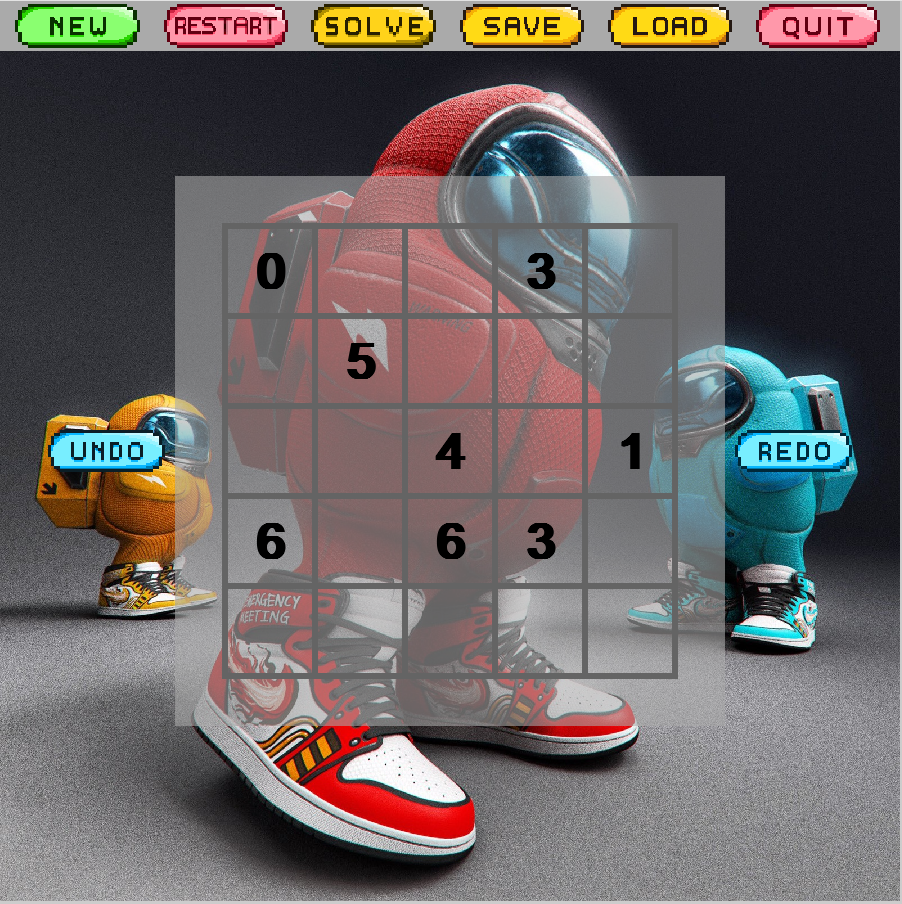
\includegraphics[height=10cm]{game.png}
    \section{Le code}
        \subsection{réduction}
            certaines fonctions était beaucoup trop longues, avec une série de switch casqe qui faisait plus de 40 lignes. 
            Grace à une liste, il à était racourci à 4 lignes :
            \begin{lstlisting}[language=c, numbers=left, frame=single]
int mov_i[9] = {0, -1, 1, 0, 0, -1, -1, 1, 1};
int mov_j[9] = {0, 0, 0, -1, 1, -1, 1, -1, 1};
i = ((signed int)i + mov_i[dir]);
j = ((signed int)j + mov_j[dir]);
            \end{lstlisting}
            \clearpage
        \subsection{solveur}
            Le plus grand obstacle auquel j'ai fait face dans la programmation du jeu, c'est le solveur. en effet, un jeu 5x5 à $2^{25}$ possibilités.
            Après de nombreuses épreuves, j'ai réussi à réduire le nombre de possibilité au nombre de victoire possible, soit 1 dans le jeu ci-dessus~(\ref{game})

    \bibliographystyle{plain}
    \bibliography{biblio}
        

\end{document}